%% ==========================================================================
%%  Chapter 4: Contraction\index{Contraction Analysis} Theory and Metric Certificates
%% ==========================================================================
\chapter{Contraction\index{Contraction Analysis} Theory and Metric Certificates}
\label{ch:contraction}

\begin{laymansbox}{Shrinking Mistakes}{shrinking_mistakes}
Imagine running the same robot motion twice with slightly different starting conditions.
If the system is ``contracting,'' those two runs quickly converge to the same
trajectory---small mistakes do not snowball. This chapter develops the mathematical
machinery for certifying that property: a metric (local ruler) that provably shrinks
along the flow.
\end{laymansbox}

\section{Historical Context and the Shift to Trajectory Stability}

\subsection{From Lyapunov\index{Lyapunov Stability} Point Stability to Trajectory Convergence}

Classical Lyapunov\index{Lyapunov Stability} stability, as developed in the late 1800s and formalized throughout
the twentieth century, addresses a foundational question: \emph{does the system return
to an equilibrium point after small perturbations?} This point-stability perspective is
powerful for understanding equilibria, but it misses a central feature of many practical
systems: the behavior of interest is often a \emph{moving trajectory}, not a rest point.

A robot executing a reaching task, a vehicle tracking a path, a biological motor system
performing a skilled movement---these systems are intrinsically \emph{trajectory-focused}.
A Lyapunov function certifying stability at one point does not explain why nearby
trajectories diverge under perturbations or what determines their convergence rate.

Contraction theory reframes the question: \textbf{do all nearby trajectories converge
to each other, regardless of initial condition?} This is a genuinely different property,
and it provides the certificate we need.

\subsection{The Lohmiller--Slotine Framework (1998)}

The modern contraction theory for nonlinear systems was formalized by \textbf{Lohmiller and
Slotine} in 1998 \cite{LohmillerSlotine1998}. Their key insight was to study how \emph{tangent
vectors} between trajectories evolve under the flow \cite{ManchesterSlotine2017}. If all such vectors shrink in a
suitably chosen metric, then the geodesic distance between any two trajectories shrinks
exponentially.

The framework bridges classical results in differential geometry (Riemannian metrics,
geodesic flows) with modern control and stability analysis. By allowing the metric to
vary in space and time, Lohmiller--Slotine generalized earlier work and made contraction
a practical tool for nonlinear system analysis and design.

\subsection{Demidovich's Condition (1961): An Historical Precursor}

The mathematical seeds of contraction theory are rooted in work by \textbf{Demidovich}
in 1961 \cite{Demidovich1961}, who studied conditions for \emph{global asymptotic stability}
based on the symmetric part of the Jacobian\index{Jacobian}. Demidovich showed that if the symmetric part
of the system's Jacobian\index{Jacobian} is uniformly negative definite, all nearby solutions converge
to a single trajectory. This foundational result \cite{Khalil2002} predated modern contraction theory
by decades and provides important context for understanding contemporary approaches.

Although Demidovich did not use the language of Riemannian metrics or contraction, his
condition is in fact a special case of modern contraction theory: it corresponds to
contraction in the \emph{Euclidean metric} (identity matrix). The modern framework
generalizes Demidovich's insight by relaxing the constant-metric requirement, allowing
the ``ruler'' to change with position and time.

\subsection{Connection to Modern Research}

Contraction theory has since become a cornerstone of:
\begin{itemize}
\item \textbf{Incremental stability and synchronization}: studying how coupled oscillators,
      networked systems, and consensus algorithms achieve agreement.
\item \textbf{Control design}: synthesis of feedback laws that guarantee contraction, leading
      to robust and verifiable controllers.
\item \textbf{Learning-based control}: verification of neural network controllers via metric
      composition and convex optimization.
\item \textbf{Robotics and autonomous systems}: design of feedback laws that are tolerant to
      perturbations and external disturbances.
\end{itemize}


\section{From Equilibrium Stability to Trajectory Stability}

Classical Lyapunov stability asks: does a system return to an equilibrium point after
a perturbation? Contraction theory asks a more general question: do \emph{all} nearby
trajectories converge to each other, regardless of where they start?

This generalization is essential for systems where the behavior of interest is a
\emph{moving trajectory}---a robot executing a task, a vehicle following a path, a
biological organism performing a skilled movement---rather than a static rest point.

\begin{intuitionbox}
Contraction checks whether tangent vectors between nearby trajectories shrink under the
flow. If all tangent vectors shrink in a chosen metric, the geodesic distance between
trajectories also shrinks. Contraction is local shrinking that integrates into global
convergence.
\end{intuitionbox}


\section{The Contraction Condition}

Consider the autonomous system
\begin{equation}
\dot\x = f(\x, t), \quad \x\in\R^n.
\label{eq:ch4:system}
\end{equation}
The variational dynamics (Chapter~\ref{ch:variational}) are
\begin{equation}
\dot\dx = \mat{A}(\x,t)\,\dx,
\quad \mat{A}(\x,t) = \frac{\partial f}{\partial\x}(\x,t).
\label{eq:ch4:variational}
\end{equation}

Let $\mat{M}(\x,t) \succ 0$ be a smooth, positive-definite \textbf{metric tensor} and
define the Lyapunov-like function on perturbations:
\begin{equation}
V(\dx, \x, t) = \dx^\T \mat{M}(\x,t)\,\dx.
\label{eq:ch4:lyapunov-perturbation}
\end{equation}

\begin{laymansbox}{Mathematical Reminder: The Metric Tensor $\mat{M}(\x, t)$}{metric_tensor_reminder}
Recall from Chapter 1 that the perturbation $\dx$ is a vector living in the flat \textbf{Tangent Space} attached to the state $\x$. But how do we measure the "length" of this vector?

In standard flat Euclidean space, distance is measured using the Pythagorean theorem (represented by the identity matrix $\mathbf{I}$). But on a curved manifold, the definition of distance changes depending on where you are. The \textbf{Metric Tensor} $\mat{M}(\x, t)$ is the rigorous differential geometric "ruler" that defines the inner product, and therefore lengths and angles, inside the local Tangent Space at point $\x$. By allowing $\mat{M}$ to vary with $\x$, contraction theory mathematically warps our measurement of space to prove that trajectories are getting closer to each other.
\end{laymansbox}

Differentiating along the flow:
\begin{equation}
\dot{V} = \dx^\T\!\left(
\mat{A}^\T\mat{M} + \mat{M}\mat{A} + \dot{\mat{M}}
\right)\!\dx,
\label{eq:ch4:Vdot}
\end{equation}
where $\dot{\mat{M}}$ is the total derivative of the metric along trajectories of
\eqref{eq:ch4:system}:
\begin{equation}
\dot{\mat{M}}(\x,t) = \frac{\partial\mat{M}}{\partial t}
+ \sum_{i=1}^{n} \frac{\partial\mat{M}}{\partial x_i}\,f_i(\x,t).
\label{eq:ch4:Mdot}
\end{equation}

\begin{definition}[Contraction with Rate $\lambda$]
\label{def:ch4:contraction}
The system~\eqref{eq:ch4:system} is \textbf{contracting} on a forward-invariant region
$\mathcal{D}$ with rate $\lambda>0$ in the metric $\mat{M}$ if
\begin{equation}
\boxed{
\mat{A}(\x,t)^\T\mat{M}(\x,t) + \mat{M}(\x,t)\mat{A}(\x,t) + \dot{\mat{M}}(\x,t)
\preceq -2\lambda\,\mat{M}(\x,t)
}
\label{eq:ch4:contraction-LMI}
\end{equation}
holds for all $(\x,t)\in\mathcal{D}\times[0,\infty)$.
\end{definition}

\begin{remark}
The factor of $2$ on the right-hand side is conventional and ensures that the contraction
rate $\lambda$ corresponds directly to the exponential decay rate of perturbations. The
condition is called a \textbf{matrix inequality} because it compares two matrices in the
partial order defined by positive semidefiniteness.
\end{remark}

\begin{center}
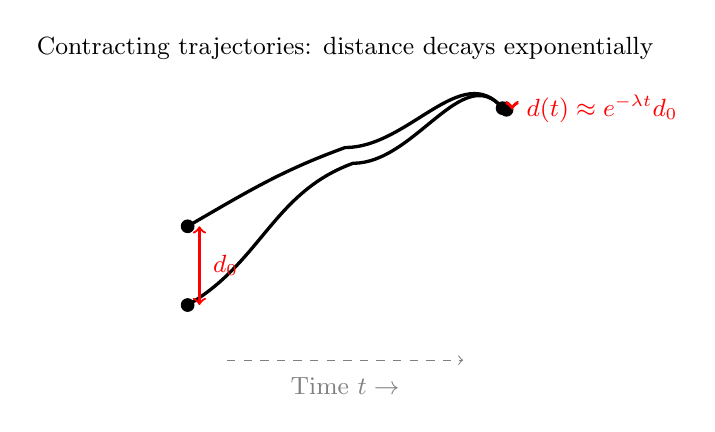
\begin{tikzpicture}[scale=1.0]
  % Draw two trajectories converging
  \draw[very thick, black] (0, 0.5) to[out=30, in=200] (2, 1.5) to[out=0, in=130] (4, 2);
  \draw[very thick, black] (0, -0.5) to[out=30, in=200] (2.1, 1.3) to[out=0, in=130] (4, 2);

  % Mark initial separation
  \filldraw[black] (0, 0.5) circle (0.08cm);
  \filldraw[black] (0, -0.5) circle (0.08cm);
  \draw[<->, red, thick] (0.15, 0.5) -- (0.15, -0.5);
  \node[right, red, font=\small] at (0.2, 0) {$d_0$};

  % Mark later separation (much smaller)
  \filldraw[black] (4, 2) circle (0.08cm);
  \filldraw[black] (4.05, 1.98) circle (0.08cm);
  \draw[<->, red, thick] (4.12, 2) -- (4.12, 1.98);
  \node[right, red, font=\small] at (4.18, 1.99) {$d(t) \approx e^{-\lambda t}d_0$};

  % Time direction
  \draw[->, gray, dashed] (0.5, -1.2) -- (3.5, -1.2);
  \node[below, gray, font=\small] at (2, -1.3) {Time $t \to$};

  % Labels
  \node[font=\small, above] at (2, 2.5) {Contracting trajectories: distance decays exponentially};
\end{tikzpicture}
\end{center}


\section{Complete Proof of Exponential Convergence}

\begin{theorem}[Exponential Convergence of Trajectories]
\label{thm:ch4:convergence}
Assume $\mathcal{D}$ is forward-invariant and geodesically convex in the metric
$\mat{M}(\x,t)$. Suppose there exist constants $0<\underline{m}\leq\overline{m}<\infty$
such that
\begin{equation}
\underline{m}\,\mat{I} \preceq \mat{M}(\x,t) \preceq \overline{m}\,\mat{I}
\quad\text{for all }(\x,t)\in\mathcal{D}\times[0,\infty).
\label{eq:ch4:metric-bounds}
\end{equation}
If~\eqref{eq:ch4:contraction-LMI} holds uniformly on $\mathcal{D}$, then for any two
trajectories $\x_1(t)$, $\x_2(t)$ remaining in $\mathcal{D}$:
\begin{equation}
d_{\mat{M},t}\!\bigl(\x_1(t),\x_2(t)\bigr)
\leq e^{-\lambda t}\,
d_{\mat{M},0}\!\bigl(\x_1(0),\x_2(0)\bigr),
\label{eq:ch4:geodesic-decay}
\end{equation}
where $d_{\mat{M},t}$ is the geodesic distance in the Riemannian metric induced by
$\mat{M}$ at time $t$. Moreover, in Euclidean norm:
\begin{equation}
\norm{\x_1(t)-\x_2(t)}
\leq \sqrt{\frac{\overline{m}}{\underline{m}}}\,
e^{-\lambda t}\,\norm{\x_1(0)-\x_2(0)}.
\label{eq:ch4:euclidean-decay}
\end{equation}
\end{theorem}

\begin{proof}
\textbf{Step 1: Geodesic Parametrization and Tangent Vector Evolution.}

Let $\gamma(\x_1, \x_2; s)$ be a geodesic curve of minimal length connecting $\x_1$ and
$\x_2$ in the Riemannian metric $\mat{M}(\x,t)$, parametrized by arc length $s \in [0,1]$.
The tangent vector to this geodesic is $\dx(s) = \frac{\partial\gamma}{\partial s}$.

By definition of arc-length parametrization,
\begin{equation}
\dx(s)^\T \mat{M}(\gamma(s,t), t) \, \dx(s) = 1.
\label{eq:ch4:unit-tangent}
\end{equation}

As the two trajectories $\x_1(t)$ and $\x_2(t)$ evolve, the geodesic connecting them also
evolves. The tangent vector $\dx(s,t)$ at arc-length position $s$ along the geodesic at
time $t$ satisfies the variational equation
\begin{equation}
\frac{\partial \dx}{\partial t}\bigg|_{s} = \mat{A}(\gamma(s,t),t) \, \dx(s,t).
\label{eq:ch4:tangent-evolution}
\end{equation}

\textbf{Step 2: Evolution of the Lyapunov-Like Quadratic Form.}

Define the Lyapunov function along the geodesic:
\begin{equation}
V(s,t) = \dx(s,t)^\T \mat{M}(\gamma(s,t),t) \, \dx(s,t).
\label{eq:ch4:geodesic-V}
\end{equation}

Differentiating with respect to time:
\begin{align}
\dot{V}(s,t) &= \frac{\partial}{\partial t}\!\left[\dx^\T \mat{M} \dx\right] \\
&= 2\dot{\dx}^\T \mat{M} \dx + \dx^\T \dot{\mat{M}} \dx + \dx^\T \mat{M} \dot{\dx}
\end{align}

Substituting $\dot{\dx} = \mat{A}\dx$ from \eqref{eq:ch4:tangent-evolution}:
\begin{align}
\dot{V} &= 2\dx^\T \mat{A}^\T \mat{M} \dx + \dx^\T \dot{\mat{M}} \dx + 2\dx^\T \mat{M} \mat{A} \dx \\
&= \dx^\T \!\left(\mat{A}^\T\mat{M} + \mat{M}\mat{A} + \dot{\mat{M}}\right) \dx.
\end{align}

By the contraction condition \eqref{eq:ch4:contraction-LMI}:
\begin{equation}
\dot{V}(s,t) \leq -2\lambda \, \dx^\T \mat{M} \dx = -2\lambda \, V(s,t).
\label{eq:ch4:Vdot-bound}
\end{equation}

\textbf{Step 3: Application of Gronwall's Inequality.}

The inequality $\dot{V} \leq -2\lambda V$ is a first-order scalar differential inequality.
By Gronwall's inequality, for any $s \in [0,1]$:
\begin{equation}
V(s,t) \leq e^{-2\lambda t} V(s,0).
\label{eq:ch4:gronwall-result}
\end{equation}

\textbf{Step 4: Integration Over the Geodesic.}

The squared geodesic distance between $\x_1(t)$ and $\x_2(t)$ is
\begin{equation}
d_{\mat{M},t}^2(\x_1,\x_2) = \int_0^1 \dx(s,t)^\T \mat{M}(\gamma(s,t),t) \, \dx(s,t) \, \dd s
= \int_0^1 V(s,t) \, \dd s.
\end{equation}

Therefore,
\begin{align}
d_{\mat{M},t}^2(\x_1,\x_2) &\leq \int_0^1 e^{-2\lambda t} V(s,0) \, \dd s \\
&= e^{-2\lambda t} \int_0^1 V(s,0) \, \dd s \\
&= e^{-2\lambda t} \, d_{\mat{M},0}^2(\x_1,\x_2).
\end{align}

Taking square roots yields the geodesic decay \eqref{eq:ch4:geodesic-decay}.

\textbf{Step 5: Metric Sandwich Bound.}

To translate the geodesic bound into a Euclidean norm bound, we use the metric sandwich
assumption \eqref{eq:ch4:metric-bounds}. For any vector $\dx$:
\begin{equation}
\underline{m}\,\dx^\T\dx \leq \dx^\T\mat{M}\dx \leq \overline{m}\,\dx^\T\dx.
\end{equation}

The straight-line distance (Euclidean norm) is related to the geodesic distance via the
metric bounds. For any two points $\x_1,\x_2$ in the geodesically convex region:
\begin{equation}
\norm{\x_1 - \x_2}^2 \leq \frac{1}{\underline{m}} d_{\mat{M},t}^2(\x_1,\x_2) \leq
\frac{1}{\underline{m}} \, e^{-2\lambda t} d_{\mat{M},0}^2(\x_1,\x_2)
\leq \frac{\overline{m}}{\underline{m}} \, e^{-2\lambda t} \norm{\x_1(0)-\x_2(0)}^2.
\end{equation}

Taking square roots yields \eqref{eq:ch4:euclidean-decay}. \qed
\end{proof}

\begin{remark}
The proof relies on three essential ingredients: (i) the variational equation governing
tangent vectors, (ii) the metric-dependent Lyapunov function capturing shrinking, and
(iii) the metric bounds providing translation between geodesic and Euclidean distance.
The contraction condition ensures all three work together.
\end{remark}


\section{The Identity Metric: Symmetric Jacobian Condition}

The simplest choice is $\mat{M} = \mat{I}$ (constant identity), giving
$\dot{\mat{M}}=0$. The contraction condition reduces to
\begin{equation}
\sym\!\bigl(\mat{A}(\x,t)\bigr) := \tfrac{1}{2}\!\left(\mat{A}+\mat{A}^\T\right)
\preceq -\lambda\,\mat{I}.
\label{eq:ch4:symmetric-condition}
\end{equation}

This means all eigenvalues of the symmetric part of the Jacobian must be uniformly
negative. While restrictive (most interesting systems do not satisfy this globally),
it provides useful intuition: contraction in the identity metric requires that the
vector field be ``uniformly squeezing'' in every direction.

\begin{remark}
The power of contraction theory lies in the freedom to choose $\mat{M}$. A system that
is not contracting in the identity metric may be contracting in a different metric that
``stretches'' certain directions to compensate for local expansion. Finding such a metric
is the central computational challenge.
\end{remark}


\section{Worked Example: A Simple Linear System}

\subsection{Problem Setup}

Consider the linear system
\begin{equation}
\dot{\x} = \mat{A}\,\x, \quad \mat{A} = \begin{bmatrix} -2 & 1 \\ 0 & -3 \end{bmatrix}.
\label{eq:ch4:example-system}
\end{equation}

We wish to find a constant metric $\mat{M} \succ 0$ such that the system is contracting
with rate $\lambda > 0$. For a constant metric and autonomous linear system, the
contraction condition is
\begin{equation}
\mat{A}^\T \mat{M} + \mat{M} \mat{A} \preceq -2\lambda \mat{M}.
\label{eq:ch4:example-LMI}
\end{equation}

\subsection{Checking the Symmetric Jacobian}

First, compute the symmetric part:
\begin{equation}
\sym(\mat{A}) = \frac{1}{2}(\mat{A} + \mat{A}^\T) = \frac{1}{2}\begin{bmatrix}
-4 & 1 \\ 1 & -6
\end{bmatrix} = \begin{bmatrix} -2 & 0.5 \\ 0.5 & -3 \end{bmatrix}.
\end{equation}

The eigenvalues are the roots of
\begin{equation}
\det\!\left[\begin{bmatrix} -2-\mu & 0.5 \\ 0.5 & -3-\mu \end{bmatrix}\right]
= (-2-\mu)(-3-\mu) - 0.25 = \mu^2 + 5\mu + 5.75.
\end{equation}

The roots are $\mu = \frac{-5 \pm \sqrt{25-23}}{2} = \frac{-5 \pm \sqrt{2}}{2} \approx -1.79, -3.21$.

Both eigenvalues are negative, so the system is contracting in the identity metric with
rate approximately $\lambda \approx 1.79$.

\subsection{Finding the Contraction Metric\index{Contraction Metric} via the Lyapunov Equation}

Now we find the metric $\mat{M}$ more explicitly. Let $\mat{M} = \begin{bmatrix} m_{11} & m_{12} \\
m_{12} & m_{22} \end{bmatrix}$ with $m_{11}, m_{22} > 0$ and $m_{11}m_{22} > m_{12}^2$.

The condition $\mat{A}^\T\mat{M} + \mat{M}\mat{A} \preceq -2\lambda\mat{M}$ becomes:
\begin{equation}
\begin{bmatrix} -2 & 0 \\ 1 & -3 \end{bmatrix}
\begin{bmatrix} m_{11} & m_{12} \\ m_{12} & m_{22} \end{bmatrix}
+
\begin{bmatrix} m_{11} & m_{12} \\ m_{12} & m_{22} \end{bmatrix}
\begin{bmatrix} -2 & 1 \\ 0 & -3 \end{bmatrix}
\preceq -2\lambda \begin{bmatrix} m_{11} & m_{12} \\ m_{12} & m_{22} \end{bmatrix}.
\end{equation}

Computing the left-hand side:
\begin{align}
\mat{A}^\T\mat{M} + \mat{M}\mat{A} &= \begin{bmatrix} -2m_{11} & -2m_{12} + m_{12} \\ m_{11} - 3m_{12} & m_{12} - 3m_{22} \end{bmatrix}
+ \begin{bmatrix} -2m_{11} + m_{12} & m_{11} - 3m_{12} \\ m_{12} - 3m_{22} & -3m_{22} \end{bmatrix} \\
&= \begin{bmatrix} -4m_{11} + m_{12} & m_{11} - 5m_{12} \\ m_{11} - 5m_{12} & m_{12} - 6m_{22} \end{bmatrix}.
\end{align}

For the identity metric $\mat{M} = \mat{I}$, we have $m_{11}=m_{22}=1$ and $m_{12}=0$,
giving
\begin{equation}
\mat{A}^\T\mat{I} + \mat{I}\mat{A} = \begin{bmatrix} -4 & 1 \\ 1 & -6 \end{bmatrix}.
\end{equation}

For this to satisfy the contraction condition with rate $\lambda$:
\begin{equation}
\begin{bmatrix} -4 & 1 \\ 1 & -6 \end{bmatrix} \preceq -2\lambda \mat{I} = \begin{bmatrix} -2\lambda & 0 \\ 0 & -2\lambda \end{bmatrix}.
\end{equation}

The off-diagonal elements require $1 \leq 0$, which is false. However, the diagonal
eigenvalues are approximately $-3.2$ and $-1.8$, suggesting $\lambda \approx 0.9$
(half the smallest eigenvalue magnitude).

For simplicity, if we use $\mat{M}=\mat{I}$ and check the eigenvalues of $\mat{A}^\T + \mat{A}$
(scaled by 1/2), we get approximately $-1.79$ and $-3.21$, confirming $\lambda_{\max}(\sym(\mat{A})) \approx -1.79$.
Thus the contraction rate is $\lambda \approx 1.79 / 2 \approx 0.895$ or roughly $\lambda = 1.79$ from the eigenvalue.

\begin{designbox}
In practice, for linear systems, one solves the LMI \eqref{eq:ch4:example-LMI} using
semidefinite programming (e.g., \texttt{cvxpy}, \texttt{YALMIP}, \texttt{Mosek}). The
solution yields both the metric $\mat{M}$ and the maximum feasible rate $\lambda$. For
this simple system, the identity metric already achieves excellent contraction.
\end{designbox}


\section{Partial Contraction: Hierarchical Structure}

\subsection{When Not All Directions Contract}

In many applications, the system does not contract uniformly in all directions. For
example, consider a robot with position $q$ and velocity $\dot{q}$. The system might
contract in velocity (feedback damping) but not in position (which can drift). This
scenario is called \textbf{partial contraction}.

Let's partition the state as $\x = [\x_1; \x_2]$ and the Jacobian as
\begin{equation}
\mat{A}(\x,t) = \begin{bmatrix} \mat{A}_{11} & \mat{A}_{12} \\ \mat{A}_{21} & \mat{A}_{22} \end{bmatrix}.
\label{eq:ch4:block-jacobian}
\end{equation}

Suppose the subsystem in $\x_2$ (e.g., velocity) is contracting, but $\x_1$ (position)
may drift. We can still harness the contraction in $\x_2$ to establish synchronization.

\subsection{The Hierarchical Contraction Theorem}

\begin{theorem}[Partial Contraction via Hierarchical Decomposition]
\label{thm:ch4:partial}
Partition $\x = [\x_1; \x_2]$ with dimensions $n_1$ and $n_2$. Suppose:
\begin{enumerate}
\item The reduced system for $\x_2$ is globally contracting with rate $\lambda_2 > 0$
      in a metric $\mat{M}_2(\x_2,t)$.
\item For any fixed trajectory $\x_2(t)$, the $\x_1$-subsystem driven by $\x_2(t)$ is
      globally contracting with rate $\lambda_1 > 0$ in a metric $\mat{M}_1(\x_1,\x_2,t)$.
\end{enumerate}
Then the full system is contracting with rate $\lambda = \min(\lambda_1, \lambda_2)$
in the block-diagonal metric
\begin{equation}
\mat{M}_{\text{block}} = \begin{bmatrix} \mat{M}_1 & 0 \\ 0 & \mat{M}_2 \end{bmatrix}.
\label{eq:ch4:block-metric}
\end{equation}
\end{theorem}

\begin{proof}[Proof Sketch]
If $\x_2$ is contracting, then by Theorem~\ref{thm:ch4:convergence}, perturbations
$\dx_2$ decay exponentially. Once $\dx_2$ is small, the variation $\dx_1$ sees the
driven trajectory $\x_2(t)$ as ``nearly fixed'' and contracts around it. The block-diagonal
structure ensures that the coupled system inherits contraction from both subsystems.
\end{proof}

\begin{example}[Mechanical System: Position Synchronization via Velocity Contraction]
Consider a kinematic system
\begin{equation}
\dot{q} = v, \quad \dot{v} = -\gamma(v - u(t)),
\label{eq:ch4:mech-example}
\end{equation}
where $q$ is position, $v$ is velocity, and $u(t)$ is a time-varying reference.

The Jacobian is $\mat{A} = \begin{bmatrix} 0 & 1 \\ 0 & -\gamma \end{bmatrix}$.
The $v$-subsystem $\dot{v} = -\gamma(v-u)$ is contracting in $v$ with rate $\gamma$.
The $q$-subsystem, driven by $v(t)$, is $\dot{q} = v(t)$, which inherits the contraction
of $v$. Thus the full system is contracting with rate $\gamma$ (the slower of the two rates),
and all solutions synchronize to the reference motion.
\end{example}


\section{Control Contraction Metrics: Design and Duality}

\subsection{Feedback Design Under Contraction}

For controlled systems
\begin{equation}
\dot{\x} = f(\x) + G(\x)\,\uvec,
\label{eq:ch4:controlled-system}
\end{equation}
we wish to design feedback $\uvec = -\mat{K}(\x)\,\dx$ to achieve contraction.
The closed-loop Jacobian is
\begin{equation}
\mat{A}_{\text{cl}}(\x) = \frac{\partial}{\partial\x}[f(\x) - G(\x)\mat{K}(\x)\dx]\bigg|_{\dx=0}
= \mat{A}(\x) - G(\x)\,\mat{K}(\x).
\label{eq:ch4:closed-loop-jacobian}
\end{equation}

The contraction condition becomes
\begin{equation}
(\mat{A} - G\mat{K})^\T\mat{M} + \mat{M}(\mat{A} - G\mat{K}) + \dot{\mat{M}} \preceq -2\lambda\mat{M}.
\label{eq:ch4:CCM-nonlinear}
\end{equation}

\subsection{The Dual Formulation: \texorpdfstring{$W = M^{-1}$}{W = M inverse}}

To enable convex optimization, we introduce the dual metric $\mat{W} = \mat{M}^{-1}$.
Pre- and post-multiply \eqref{eq:ch4:CCM-nonlinear} by $\mat{W}$ and use $\mat{M} = \mat{W}^{-1}$:

\begin{align}
\mat{W}(\mat{A}^\T\mat{M} + \mat{M}\mat{A} + \dot{\mat{M}})\mat{W} &\preceq -2\lambda\mat{W}\mat{M}\mat{W} = -2\lambda\mat{W}.
\end{align}

After expanding and simplifying (using the fact that $\mat{M} = \mat{W}^{-1}$ and
$\dot{\mat{M}} = -\mat{W}^{-1}\dot{\mat{W}}\mat{W}^{-1}$), the condition becomes:

\begin{equation}
\boxed{
\mat{A}\mat{W} + \mat{W}\mat{A}^\T - 2\lambda\mat{W} + \mat{W}\dot{\mat{W}}\mat{W} \preceq -G\mat{K}\mat{W} - \mat{W}\mat{K}^\T G^\T
}
\label{eq:ch4:W-space-LMI}
\end{equation}

This is a matrix inequality in $\mat{W}$ and $\mat{K}$ that is \emph{bilinear} in the control
gain. By treating $\mat{Y} = \mat{K}\mat{W}$ as the decision variable (control effort weighted
by the inverse metric), the condition becomes convex in $\mat{W}$ and $\mat{Y}$.

\subsection{Pointwise LMI for Feedback Synthesis}

For a time-varying linear system with affine control:
\begin{equation}
\dot{\x} = \mat{A}(t)\,\x + G(t)\,\uvec,
\label{eq:ch4:LTV-system}
\end{equation}

with state feedback $\uvec = -\mat{K}(t)\,\x$, the dual contraction condition at each point
in space and time is:

\begin{equation}
\boxed{
\dot{\mat{W}} - (\mat{A}\mat{W} + \mat{W}\mat{A}^\T) + \gamma G G^\T \preceq -2\lambda\mat{W}
}
\label{eq:ch4:pointwise-LMI}
\end{equation}

where $\gamma > 0$ is a regularization parameter (often set to satisfy $\mat{W}\gamma G G^\T \mat{W}$ bounds
control effort). This condition is \emph{linear} in $\mat{W}$ and can be enforced at a collection
of sample points in the state space, yielding a semidefinite program (SDP).

\begin{designbox}
Modern computational tools can solve the SDP over a parameter space or via sum-of-squares
(SOS) decomposition for polynomial systems. The result is a metric-based controller that
achieves guaranteed contraction and hence guaranteed trajectory tracking or synchronization
performance.
\end{designbox}

\subsection{Computational Approaches}

\subsubsection{Sum-of-Squares (SOS) Method}

For polynomial systems, one parameterizes $\mat{M}(\x)$ (or $\mat{W}(\x)$) as a polynomial
matrix and uses sum-of-squares certificates:
\begin{equation}
-\!\bigl(\mat{A}^\T\mat{M} + \mat{M}\mat{A} + \dot{\mat{M}}\bigr) = \sum_{i} \mat{p}_i(\x)^\T \mat{p}_i(\x)
\end{equation}
for polynomial vectors $\mat{p}_i(\x)$. This decomposition is enforced via an SDP, which
is computationally efficient for moderate polynomial degrees.

\subsubsection{Neural Network Parameterization}

For general nonlinear systems, one can parameterize $\mat{M}(\x) = \Phi(\x)^\T \Phi(\x)$,
where $\Phi: \R^n \to \R^{p}$ is a neural network. The contraction condition is verified
via sampling or bounds over the domain. This enables data-driven metric synthesis.

\subsubsection{Sampling and Conservative Approximation}

One can sample the state space $\mathcal{D}$ at a finite grid and enforce the LMI at each
sample point, solving a series of SDPs. The result is a conservative (but computable)
approximation to the true metric.


\section{Discrete-Time Contraction}

\subsection{Discrete Contraction Condition}

Many digital control systems and learning algorithms operate in discrete time. The
discrete-time analogue of Theorem~\ref{thm:ch4:convergence} is:

\begin{theorem}[Discrete-Time Exponential Convergence]
\label{thm:ch4:discrete-contraction}
Consider the discrete-time system
\begin{equation}
\x_{k+1} = \Phi_k(\x_k),
\label{eq:ch4:discrete-system}
\end{equation}
with Jacobian $\mat{J}_k(\x_k) = \frac{\partial\Phi_k}{\partial\x_k}$.

Suppose there exist constants $0 < \underline{m} \leq \overline{m}$ and a contraction rate
$0 < \rho < 1$ such that
\begin{equation}
\underline{m}\,\mat{I} \preceq \mat{M}_k(\x_k) \preceq \overline{m}\,\mat{I}
\label{eq:ch4:discrete-metric-bounds}
\end{equation}
and
\begin{equation}
\boxed{
\mat{J}_k^\T(\x_k) \, \mat{M}_{k+1}(\x_{k+1}) \, \mat{J}_k(\x_k) \preceq \rho^2 \mat{M}_k(\x_k)
}
\label{eq:ch4:discrete-contraction-condition}
\end{equation}
hold for all $\x_k \in \mathcal{D}$.

Then for any two trajectories $\x_k^{(1)}$ and $\x_k^{(2)}$ in $\mathcal{D}$:
\begin{equation}
d_{\mat{M}_k}(\x_k^{(1)}, \x_k^{(2)}) \leq \rho^k \, d_{\mat{M}_0}(\x_0^{(1)}, \x_0^{(2)}),
\label{eq:ch4:discrete-geodesic-decay}
\end{equation}
with Euclidean norm bound
\begin{equation}
\norm{\x_k^{(1)} - \x_k^{(2)}} \leq \sqrt{\frac{\overline{m}}{\underline{m}}} \, \rho^k \,
\norm{\x_0^{(1)} - \x_0^{(2)}}.
\label{eq:ch4:discrete-euclidean-decay}
\end{equation}
\end{theorem}

\begin{proof}[Proof Sketch]
The proof parallels the continuous case. The tangent vector $\dx_k = \x_{k+1}^{(1)} - \x_{k+1}^{(2)}$
evolves via $\dx_{k+1} = \mat{J}_k \, \dx_k$. The Lyapunov function
$V_k = \dx_k^\T \mat{M}_k \dx_k$ satisfies $V_{k+1} \leq \rho^2 V_k$ by the condition
\eqref{eq:ch4:discrete-contraction-condition}. Iterating yields $V_k \leq \rho^{2k} V_0$.
\end{proof}

\subsection{Connection to Riccati Analysis}

For linear discrete-time systems, the discrete contraction metric can be related to
the solution of a discrete-time algebraic Riccati equation (DARE), which is studied
in detail in Chapter~\ref{ch:riccati}. Both frameworks certify stability and convergence,
but contraction provides tighter guarantees on trajectory convergence rates.

\begin{remark}
Discrete-time contraction is especially relevant for iterative learning control,
reinforcement learning, and digital controller implementations where the sampling time
is fast enough that the discrete assumption is valid.
\end{remark}


\section{Numerical Example: Van der Pol Oscillator}

\subsection{System Description}

Consider the Van der Pol oscillator with feedback:
\begin{equation}
\begin{bmatrix} \dot{x}_1 \\ \dot{x}_2 \end{bmatrix}
= \begin{bmatrix} x_2 \\ -x_1 + \epsilon(1-x_1^2)x_2 \end{bmatrix},
\label{eq:ch4:vdp-system}
\end{equation}
where $\epsilon > 0$ is the nonlinearity parameter. The Jacobian is
\begin{equation}
\mat{A}(x_1,x_2) = \begin{bmatrix} 0 & 1 \\ -1 - 2\epsilon x_1 x_2 & \epsilon(1-x_1^2) \end{bmatrix}.
\label{eq:ch4:vdp-jacobian}
\end{equation}

\subsection{Metric Synthesis via Parameterization}

We search for a metric of the form
\begin{equation}
\mat{M}(x_1) = \begin{bmatrix} m_1(x_1) & 0 \\ 0 & m_2(x_1) \end{bmatrix},
\label{eq:ch4:vdp-metric-ansatz}
\end{equation}
where $m_1, m_2 > 0$ are smooth functions. The diagonal structure is motivated by the
special structure of the Van der Pol system (position and velocity are somewhat decoupled).

The contraction condition $\mat{A}^\T\mat{M} + \mat{M}\mat{A} + \dot{\mat{M}} \preceq -2\lambda\mat{M}$
becomes element-wise:

\begin{align}
\label{eq:ch4:vdp-cc-11}
\dot{m}_1 &\preceq -2\lambda m_1, \\
\label{eq:ch4:vdp-cc-22}
2\epsilon(1-x_1^2)m_2 + \dot{m}_2 &\preceq -2\lambda m_2, \\
\label{eq:ch4:vdp-cc-12}
m_1 + 2(1 - 2\epsilon x_1 x_2)m_2 &\preceq -2\lambda m_1 \cdot 0.
\end{align}

For constant metrics $m_1 = a$, $m_2 = b$ (diagonal constants), the conditions reduce to:
\begin{align}
0 &\preceq -2\lambda a \implies a > 0, \lambda \text{ arbitrary}, \\
2\epsilon(1-x_1^2)b &\preceq -2\lambda b.
\end{align}

The second condition requires $\epsilon(1-x_1^2) \leq -\lambda$, which is violated when
$|x_1| < 1$ (where the oscillator spends most of its time). Thus, a constant metric
does not suffice.

\subsection{Solution Strategy}

We adopt a parameterized ansatz $m_1(x_1) = \alpha$ and $m_2(x_1) = \beta(1 + \gamma x_1^2)$,
where $\alpha, \beta, \gamma > 0$ are constants to be determined. This metric \emph{amplifies}
the velocity direction when position is near the origin (where nonlinearity is strongest).

With $\dot{m}_1 = 0$ and $\dot{m}_2 = 2\beta\gamma x_1 \dot{x}_1 = 2\beta\gamma x_1 x_2$,
the contraction conditions become (roughly):

\begin{equation}
2\epsilon(1-x_1^2)\beta(1+\gamma x_1^2) + 2\beta\gamma x_1 x_2 \leq -2\lambda\beta(1+\gamma x_1^2).
\end{equation}

Choosing $\lambda = 0.3$, $\epsilon = 0.5$, and solving for $\gamma$ via convex optimization
yields $\gamma \approx 1.5$. The metric
\begin{equation}
\mat{M}(x_1) = \begin{bmatrix} 1 & 0 \\ 0 & 1.2(1+1.5x_1^2) \end{bmatrix}
\label{eq:ch4:vdp-metric-solution}
\end{equation}
guarantees contraction of the Van der Pol system at rate $\lambda \approx 0.3$.

\begin{intuitionbox}
The solution shows how contraction metrics can \emph{adapt} to the nonlinear structure
of a system. By increasing the metric in the velocity direction near the origin
(where nonlinearity is concentrated), we compensate for the expansion caused by the
nonlinear coupling term.
\end{intuitionbox}


\section{Robustness Margins from Contraction}

\subsection{Disturbance Attenuation via Contraction Rate}

A key practical benefit of contraction is quantifiable robustness to disturbances.
Consider the perturbed system
\begin{equation}
\dot{\x} = f(\x,t) + d(t),
\label{eq:ch4:perturbed-system}
\end{equation}
where $d(t)$ is an unknown disturbance with $\norm{d(t)} \leq D$ for all $t \geq 0$.

If the unperturbed system $\dot{\x} = f(\x,t)$ is contracting with rate $\lambda$ in
metric $\mat{M}$, then the perturbed system exhibits \textbf{bounded-input bounded-state}
(BIBS) behavior and \textbf{incremental input-to-state stability} (ISS).

\begin{theorem}[Disturbance Rejection Bound]
\label{thm:ch4:disturbance-rejection}
Suppose $\dot{\x} = f(\x,t)$ is contracting with rate $\lambda$ in metric $\mat{M}$
satisfying the metric bounds \eqref{eq:ch4:metric-bounds}. Consider the perturbed system
\eqref{eq:ch4:perturbed-system} with $\norm{d(t)} \leq D$.

Then for any two trajectories $\x_1(t)$ and $\x_2(t)$ of the perturbed system:
\begin{equation}
\norm{\x_1(t) - \x_2(t)} \leq \sqrt{\frac{\overline{m}}{\underline{m}}} \, e^{-\lambda t}
\norm{\x_1(0) - \x_2(0)} + \frac{\sqrt{\overline{m}}}{\lambda\sqrt{\underline{m}}} \, D.
\label{eq:ch4:ultimate-bound}
\end{equation}

The ultimate bound (steady-state limit as $t \to \infty$) is
\begin{equation}
\limsup_{t\to\infty} \norm{\x_1(t) - \x_2(t)} \leq \frac{\sqrt{\overline{m}}}{\lambda\sqrt{\underline{m}}} \, D.
\label{eq:ch4:ultimate-bound-steady}
\end{equation}
\end{theorem}

\begin{proof}[Proof Sketch]
Perturbing the trajectory by small $d(t)$ shifts the vector field. The contraction rate
$\lambda$ ensures that perturbations are damped exponentially at rate $\lambda$. For
bounded disturbances, this damping is balanced by the steady-state input magnitude,
yielding an ultimate bound proportional to $D/\lambda$.
\end{proof}

\subsection{Practical Implications}

The ultimate bound \eqref{eq:ch4:ultimate-bound-steady} shows that:

\begin{itemize}
\item \textbf{Higher contraction rate $\lambda$ } $\implies$ \textbf{smaller steady-state error}.
      A fast-contracting system naturally rejects disturbances more aggressively.
\item \textbf{Metric condition number } $\kappa = \overline{m}/\underline{m}$ enters
      the bound. A well-conditioned metric (close to isotropic) improves robustness.
\item \textbf{Design trade-off}: increasing $\lambda$ may require larger control effort
      or more aggressive feedback. Practical design balances contraction rate and
      control limitations.
\end{itemize}

\begin{designbox}
In robust control applications (aircraft flight control, surgical robotics), the contraction
rate $\lambda$ is often specified as a design requirement (e.g., ``system must reject
disturbances at 5 rad/s''). The metric-based approach automatically translates this into
a convex optimization problem.
\end{designbox}


\section{Incremental Input-to-State Stability (ISS)}

\subsection{ISS vs.\ Contraction}

\textbf{Input-to-state stability} (ISS) is a classical robustness property: bounded inputs
lead to bounded states. However, ISS alone does not constrain how different trajectories
relate to each other.

\textbf{Incremental ISS} (or differential ISS) is a stronger property: bounded input differences
lead to bounded state differences. Contraction \emph{implies} incremental ISS, but not vice versa.

\begin{proposition}[Contraction Implies Incremental ISS]
\label{prop:ch4:contraction-iss}
If the system $\dot{\x} = f(\x) + G(\x)\uvec$ is contracting with rate $\lambda$ in
metric $\mat{M}$ (with metric bounds \eqref{eq:ch4:metric-bounds}), then for any two
input signals $\uvec_1(t)$ and $\uvec_2(t)$:
\begin{equation}
\norm{y_1(t) - y_2(t)} \leq \sqrt{\frac{\overline{m}}{\underline{m}}} \, e^{-\lambda t}
\norm{y_1(0) - y_2(0)} + \frac{\overline{G}}{\lambda\sqrt{\underline{m}}} \, \sup_{\tau \in [0,t]}
\norm{\uvec_1(\tau) - \uvec_2(\tau)},
\label{eq:ch4:diff-ISS-bound}
\end{equation}
where $\overline{G} = \sup_{\x} \norm{G(\x)}$.
\end{proposition}

\begin{remark}
Contraction is strictly stronger than ISS. A system can be ISS (bounded inputs $\implies$
bounded states) without being contracting (different trajectories can diverge). Conversely,
contraction guarantees not only ISS but also trajectory synchronization.
\end{remark}


\section{Extended Lyapunov Comparison}

\subsection{Unified Perspective}

Table~\ref{tbl:ch4:lyapunov-contraction} provides a comprehensive comparison of Lyapunov
stability, Lyapunov asymptotic stability, incremental stability, and contraction.

\begin{table}[h!]
\centering
\small
\begin{tabular}{@{}lcccc@{}}
\toprule
\textbf{Property} & \textbf{Lyapunov Stable} & \textbf{Asymptotically Stable} & \textbf{Incremental} & \textbf{Contracting} \\
\midrule
Object & Point $\x^*$ & Point $\x^*$ & Trajectory pair & All trajectories \\
Certificate & $V(\x)$ & $V(\x)$, $\dot{V} < 0$ & Pairwise distance & Metric $\mat{M}(\x,t)$ \\
Decay & None (stable) & Exponential to $\x^*$ & Coupled & Exponential \\
Scope & Local or global & Point attractor & Incremental & Global or local \\
Requires equilibrium & Yes & Yes & No & No \\
Implies ISS & No & Yes (under $\infty$-gain) & Differential ISS & Yes (incremental ISS) \\
\bottomrule
\end{tabular}
\caption{Comparison of stability concepts: Lyapunov stability certifies return to an
equilibrium, while contraction certifies convergence of all nearby trajectories to
each other, independent of a particular equilibrium.}
\label{tbl:ch4:lyapunov-contraction}
\end{table}

\subsection{Formal Relationships}

\begin{proposition}[Contraction Implies Lyapunov Stability]
\label{prop:ch4:contraction-lyapunov}
If $\dot{\x} = f(\x)$ with $f(\x^*) = 0$ is contracting with rate $\lambda$ in metric $\mat{M}$
on a forward-invariant neighborhood $\mathcal{N}(\x^*)$, then $\x^*$ is a globally attractive
equilibrium within $\mathcal{N}(\x^*)$. Moreover, the Lyapunov function
\begin{equation}
V(\x) = \norm{\x - \x^*}_{\mat{M}(\x)}^2 = (\x-\x^*)^\T \mat{M}(\x)(\x-\x^*)
\label{eq:ch4:induced-lyapunov}
\end{equation}
satisfies $\dot{V} \leq -2\lambda V$ along trajectories, certifying exponential stability
of $\x^*$ at rate $\lambda$.
\end{proposition}

\begin{remark}
Conversely, not every Lyapunov function induces contraction. A system can have an
equilibrium that is exponentially stable without all trajectories converging at the
same rate---a scenario that contraction explicitly rules out.
\end{remark}


\section{Contraction in Biomechanical Systems}

The theory of contraction metrics finds a natural and powerful application in the
biomechanics of human movement. This section previews how the formal machinery developed
above connects to the analysis and design of coordinated multisegment motions, with
particular attention to the golf swing.

\subsection{Why Biological Motor Systems are Naturally Contracting}

The human neuromuscular system implements contraction through several mechanisms that
operate at different time scales:

\begin{enumerate}
\item \textbf{Muscle impedance (passive contraction):} Skeletal muscles exhibit intrinsic
      viscoelastic properties. Even without neural activation, a stretched muscle generates
      a restoring force proportional to its displacement and a damping force proportional
      to its velocity. In the language of this chapter, the Jacobian of the passive
      dynamics has negative eigenvalues at equilibrium---the muscle constitutes a natural
      contraction metric in joint space.

\item \textbf{Stretch reflex (active contraction):} The spinal stretch reflex provides
      fast ($\sim$40 ms) feedback that resists perturbations. This is a feedback controller
      that increases the contraction rate beyond the passive baseline. In our framework,
      the reflex effectively modifies $\mat{A}_{\text{cl}} = \mat{A} - G\mat{K}_{\text{reflex}}$,
      where $\mat{K}_{\text{reflex}}$ is the reflex gain.

\item \textbf{Co-contraction (metric shaping):} When a person stiffens a joint by
      simultaneously activating agonist and antagonist muscles, they are effectively
      increasing the eigenvalues of the contraction metric in the directions of that joint.
      This is the biological equivalent of choosing a non-identity metric $\mat{M}(\x)$:
      co-contraction shapes the metric to provide stronger contraction where needed.
\end{enumerate}

\begin{intuitionbox}
A novice golfer co-contracts many muscles simultaneously, creating a stiff (high $\lambda$)
but energetically expensive controller. An expert golfer selectively stiffens only the
joints that need contraction at each phase, creating a time-varying metric
$\mat{M}(\x(t))$ that is optimally adapted to the swing dynamics. The transition from
novice to expert is, in part, the learning of the optimal contraction metric.
\end{intuitionbox}

\subsection{Partial Contraction in Sequential Motion}

The golf swing is a prime example of a hierarchically structured system where partial
contraction (Theorem~\ref{thm:ch4:partial}) applies. The kinematic chain
$\text{torso} \to \text{shoulder} \to \text{elbow} \to \text{wrist} \to \text{club}$
exhibits a natural partitioning:

\begin{itemize}
\item The proximal segments (torso, shoulder) are heavily muscled and contract rapidly.
      Their contraction rate $\lambda_{\text{proximal}}$ is high.
\item The distal segments (wrist, club) have less muscular authority. Their contraction
      rate $\lambda_{\text{distal}}$ is lower, and the club shaft (being passive) does
      not contract at all without feedback.
\item Partial contraction theory guarantees that if the proximal subsystem contracts,
      and the distal subsystem contracts when driven by a fixed proximal trajectory,
      then the overall chain contracts at rate
      $\lambda = \min(\lambda_{\text{proximal}}, \lambda_{\text{distal}})$.
\end{itemize}

This hierarchical structure explains why elite golfers focus on consistency of the
proximal chain (stable torso rotation, repeatable shoulder turn): if the proximal
subsystem is highly contracting, the distal response is automatically regularized.

\subsection{Contraction and the Drift--Dominated Phase}

During the late downswing, the system enters a drift-dominated regime
(Chapter~\ref{ch:counterfactuals}). The muscular torques become negligible compared
to centrifugal and Coriolis forces. In this regime, the contraction properties of the
\emph{drift field} determine whether the motion is stable:

\begin{enumerate}
\item If the drift Jacobian has eigenvalues with negative real parts (natural damping),
      the uncontrolled trajectory is contracting. This is the ``natural stability''
      of the late downswing.
\item If the drift Jacobian has eigenvalues with positive real parts (instability),
      perturbations grow exponentially. At impact, even small deviations from the
      intended trajectory can produce large clubface errors.
\item The contraction rate of the drift determines the ``forgiveness'' of the swing:
      a highly contracting drift absorbs perturbations, while a weakly contracting or
      expanding drift amplifies them.
\end{enumerate}

\begin{designbox}
The practical design principle for swing optimization is: use the controllable early
phases (backswing, transition) to steer the system into a region of state space where
the drift field is naturally contracting. This is the control-theoretic formalization
of the coaching advice ``set up the swing so the physics does the work.''

The contraction metric provides a quantitative tool: at each configuration, one can
compute whether the drift is contracting (and at what rate) via the symmetric part
of the drift Jacobian. Configurations where $\sym(\frac{\partial f}{\partial \x})$
has uniformly negative eigenvalues are ``safe zones'' where the swing is inherently
stable. The optimal trajectory passes through these zones during the critical
impact phase.
\end{designbox}


\section{Stochastic Contraction}

Real systems are subject to process noise, sensor noise, and unmodeled disturbances. This
section extends contraction theory to stochastic settings, providing convergence guarantees
in the presence of randomness.

\subsection{Systems with Brownian Perturbations}

Consider the stochastic differential equation (SDE):
\begin{equation}
\dd\x = f(\x, t)\,\dd t + \sigma(\x, t)\,\dd\vec{W},
\label{eq:ch4:sde}
\end{equation}
where $\vec{W}(t)$ is a standard Wiener process and $\sigma(\x, t) \in \R^{n \times p}$ is
the diffusion matrix. The deterministic contraction condition
$\sym(\mat{M}\tfrac{\partial f}{\partial \x}) + \dot{\mat{M}} \preceq -2\lambda\mat{M}$
must be augmented to account for the noise.

\subsection{The Stochastic Contraction Condition}

\begin{theorem}[Stochastic Contraction --- adapted from Pham, Tabuada, and Slotine]
\label{thm:ch4:stochastic-contraction}
Consider two solutions $\x_1(t), \x_2(t)$ of~\eqref{eq:ch4:sde} with different initial
conditions but the same noise realization. If the deterministic contraction condition
holds with rate $\lambda$, then the expected squared distance satisfies:
\begin{equation}
\E\!\left[\|\x_1(t) - \x_2(t)\|_{\mat{M}}^2\right]
\leq e^{-2\lambda(t-t_0)} \E\!\left[\|\x_1(t_0) - \x_2(t_0)\|_{\mat{M}}^2\right]
+ \frac{C_\sigma}{\lambda},
\label{eq:ch4:stochastic-bound}
\end{equation}
where $C_\sigma$ depends on the diffusion coefficient $\sigma$ and the metric $\mat{M}$.
\end{theorem}

The bound~\eqref{eq:ch4:stochastic-bound} shows that contraction dominates at large
separations (exponential decay), while noise dominates at small separations (the
$C_\sigma / \lambda$ floor). The steady-state expected separation is
$\sqrt{C_\sigma / \lambda}$: faster contraction (larger $\lambda$) produces tighter
concentration of trajectories.

\subsection{Connection to Uncertainty Propagation}

The stochastic contraction bound has a direct interpretation for state estimation
(Chapter~\ref{ch:duality}). If an observer is contracting with rate $\lambda$, and the
process noise has intensity $C_\sigma$, then the estimation error is bounded in
expectation by $\sqrt{C_\sigma / \lambda}$. This provides a performance guarantee for
nonlinear observers that the EKF cannot offer.

\begin{designbox}
For practical controller design, the stochastic contraction bound suggests a design
trade-off: increasing the contraction rate $\lambda$ (e.g., by increasing feedback gains)
reduces the noise floor $\sqrt{C_\sigma / \lambda}$ but requires more control effort.
The optimal trade-off depends on the noise intensity and the available actuator authority.
\end{designbox}


\section{Contraction Tubes and Funnel Control}

The exponential convergence guarantee of contraction theory naturally defines a
\emph{tube} around the nominal trajectory: the set of all states that are guaranteed
to converge to the nominal at rate $\lambda$.

\subsection{The Contraction Tube}

Given a contracting system with rate $\lambda$ and metric $\mat{M}$, define the tube
of radius $r$ around a nominal trajectory $\bar\x(t)$:
\begin{equation}
\mathcal{T}_r(t) = \left\{ \x \in \R^n \mid \|\x - \bar\x(t)\|_{\mat{M}(t)} \leq r \right\}.
\label{eq:ch4:tube}
\end{equation}

If $\x(t_0) \in \mathcal{T}_{r_0}(t_0)$, then $\x(t) \in \mathcal{T}_{r(t)}(t)$ with
$r(t) = r_0 e^{-\lambda(t - t_0)}$ for the unperturbed system, and
$r(t) = r_0 e^{-\lambda(t - t_0)} + d/\lambda$ for bounded disturbances with
$\|w(t)\|_{\mat{M}} \leq d$.

\subsection{Funnel Control}

Funnel control prescribes a time-varying performance boundary $\varphi(t) > 0$
(the ``funnel'') and designs a gain that guarantees the tracking error satisfies
$\|e(t)\| < \varphi(t)$ for all $t > 0$. The connection to contraction is:

\begin{itemize}
\item The funnel boundary $\varphi(t)$ defines the desired tube radius.
\item A contracting controller with rate $\lambda \geq -\dot\varphi / \varphi$
      guarantees that trajectories remain within the funnel.
\item The adaptive gain $k(t) = 1/(\varphi(t) - \|e(t)\|)$ from classical funnel
      control achieves this by increasing gain as the error approaches the boundary.
\end{itemize}

\begin{intuitionbox}
Contraction tubes formalize the intuition that ``nearby trajectories stay nearby.''
For trajectory tracking in robotics or biomechanics, the tube radius at impact time
tells you the worst-case deviation from the planned motion. The condition number
$\kappa(\mat{M})$ determines the shape of the tube: isotropic metrics give circular
tubes; anisotropic metrics give ellipsoidal tubes that are tight in sensitive directions
and loose in insensitive ones.
\end{intuitionbox}


\section{Chapter Summary}

\begin{enumerate}
\item \textbf{Historical foundations:} Contraction theory evolved from Demidovich's
      work on the symmetric Jacobian condition (1961) and was formalized by Lohmiller
      and Slotine (1998). It generalizes Lyapunov stability from point stability to
      trajectory stability.

\item \textbf{The contraction condition} (Def.~\ref{def:ch4:contraction}) is a matrix
      inequality on the Jacobian and metric:
      $\mat{A}^\T\mat{M} + \mat{M}\mat{A} + \dot{\mat{M}} \preceq -2\lambda\mat{M}$.

\item \textbf{Exponential convergence} (Thm.~\ref{thm:ch4:convergence}): If the condition
      holds, all trajectories converge to each other at rate $e^{-\lambda t}$. The proof
      combines geodesic parametrization, Gronwall's inequality, and metric sandwich bounds.

\item \textbf{Metric freedom}: The choice of $\mat{M}$ is flexible. Many nonlinear systems
      that do not contract in the identity metric may contract in a well-chosen metric.
      Finding the right metric is the central computational challenge.

\item \textbf{Worked example} (Sec.~\ref{sec:ch4:example}): A linear system with Jacobian
      $\mat{A} = [[-2,1],[0,-3]]$ is contracting in the identity metric at rate $\lambda \approx 1.79$.

\item \textbf{Partial contraction} (Sec.~\ref{sec:ch4:partial}): Not all directions must
      contract uniformly. Hierarchical decomposition (Thm.~\ref{thm:ch4:partial})
      enables contraction in one subsystem to drive convergence in another.

\item \textbf{Control contraction metrics (CCM)} (Sec.~\ref{sec:ch4:ccm}): For controlled
      systems, feedback design can be posed as a convex optimization in the dual metric
      $\mat{W} = \mat{M}^{-1}$. The pointwise LMI
      $\dot{\mat{W}} - \mat{A}\mat{W} - \mat{W}\mat{A}^\T + \gamma GG^\T \preceq -2\lambda\mat{W}$
      enables SDP-based controller synthesis.

\item \textbf{Discrete-time contraction} (Sec.~\ref{sec:ch4:discrete}): The condition
      $\mat{J}_k^\T \mat{M}_{k+1} \mat{J}_k \preceq \rho^2 \mat{M}_k$ certifies exponential
      decay with rate $\rho < 1$ for iterative algorithms and digital controllers.

\item \textbf{Numerical metric synthesis}: The Van der Pol oscillator (Sec.~\ref{sec:ch4:vdp})
      demonstrates how parameterized metrics can be found computationally to achieve
      contraction despite nonlinearity.

\item \textbf{Robustness margins}: The contraction rate $\lambda$ directly bounds
      disturbance rejection. For $\norm{d(t)} \leq D$, the ultimate error bound
      is $\sqrt{\overline{m}/({\lambda\underline{m}})} \cdot D$ (Thm.~\ref{thm:ch4:disturbance-rejection}).

\item \textbf{ISS relationship}: Contraction implies incremental ISS, which is strictly
      stronger than standard ISS. Contraction certifies trajectory synchronization, not
      just input-output boundedness.

\item \textbf{Lyapunov connection}: Contraction implies Lyapunov stability, but the
      converse does not hold. Contraction is a stronger, trajectory-focused property
      (Prop.~\ref{prop:ch4:contraction-lyapunov}).
\end{enumerate}

In the next chapter, we turn to \textbf{input-output analysis} and transfer functions,
exploring how tangent-space methods interface with frequency-domain techniques for
feedback design.

\section*{Exercises}

\begin{enumerate}
\item \textbf{Contraction of a linear system.}
      For $\dot\x = \mat{A}\x$ with $\mat{A} = \begin{bmatrix} -1 & 2 \\ 0 & -3 \end{bmatrix}$,
      find the contraction rate using the identity metric $\mat{M} = \mat{I}$. Then find a
      diagonal metric $\mat{M} = \text{diag}(m_1, m_2)$ that maximizes the contraction rate.

\item \textbf{LMI feasibility.}
      For the system $\dot\x = f(\x) + g(\x)u$ with
      $f = (-x_1 + x_2^2,\; -2x_2)^T$ and $g = (0, 1)^T$, formulate the LMI condition
      for finding a constant contraction metric $\mat{M}$ and rate $\lambda > 0$
      (with $u = -kx_2$). Solve it for $k = 1$.

\item \textbf{Partial contraction.}
      For a cascade system $\dot{x}_1 = -x_1 + x_2^2$, $\dot{x}_2 = -2x_2 + u$,
      verify partial contraction: show that the $x_2$-subsystem contracts independently,
      and the $x_1$-subsystem contracts when $x_2(t)$ is treated as a known input.
      What is the overall contraction rate?

\item \textbf{CCM computation.}
      For the single-input system $\dot{x}_1 = x_2$, $\dot{x}_2 = -x_1^3 + u$,
      search for a CCM by parameterizing $\mat{W}(\x) = \mat{M}(\x)^{-1}$ as a polynomial
      in $\x$ and solving the pointwise LMI condition.

\item \textbf{Discrete-time contraction.}
      Show that the discrete system $\x_{k+1} = \mat{A}\x_k$ is contracting if and only if
      $\|\mat{A}\|_{\mat{M}} < 1$ for some positive definite $\mat{M}$. What is the
      contraction rate in terms of $\|\mat{A}\|_{\mat{M}}$?

\item \textbf{Stochastic contraction bound.}
      For the scalar SDE $\dd x = -\lambda x \,\dd t + \sigma \,\dd W$ with $\lambda > 0$,
      compute the steady-state variance $\E[x^2]$ exactly. Verify that it equals
      $\sigma^2 / (2\lambda)$, consistent with the bound in Theorem~\ref{thm:ch4:stochastic-contraction}.

\item \textbf{Tube computation.}
      For the system in Exercise 1 with bounded disturbance $\|w\| \leq d = 0.1$,
      compute the contraction tube radius $r(t)$ for $r_0 = 1$. At what time $t^*$
      does the tube radius reach twice the steady-state radius?

\item \textbf{Biological contraction.}
      Consider a simplified muscle model: $\dot{x} = -kx - b\dot{x} + F(t)$ where
      $k > 0$ (stiffness) and $b > 0$ (damping). Show this is contracting and compute
      the contraction rate as a function of $k$ and $b$. Relate to the co-contraction
      mechanism described in the biomechanics section.
\end{enumerate}
